\subsection{Tumor Radiation}

As mentioned in the previous section, external beam \acs{RT} is a widespread non-invasive modality for cancer treatment with or without surgical tumor resection.
Studies indicate that it should be used in over 50\% of all cancer cases once in the course of the illness~\cite{delaney_role_2005}. 
Ionizing radiation of \ac{RT} interacts with the patient's tissue in a way that causes direct or indirect biological damage to cells.
Interaction processes release free radicals inside the tissue, which cause \ac{DNA} damage in the form of single- or double strand breaks, leading to the induction of apoptosis~\cite{kaina_dna_2003} and therefore the destruction of the radiated cell.
Healthy tissue is able to repair such \acs{DNA} damage under normal conditions. 
The repair capabilities of cancerous cells are downregulated due to the microenviromental conditions, such as hypoxia, low pH and nutrient deficiency in the primary cancer region~\cite{li_dna_2021}.
Radiation takes advantage of these down-regulated repair mechanisms, resulting in the destruction of cancer cells while limiting radiation to a point where healthy tissue can regenerate.\\
Photon attenuation is described by an exponential decay, meaning that a photon beam can not be entirely shielded.
This is of crucial importance for the optimal planning of the entire \ac{RT}.
Since tumors are usually located in deeper regions of the body (see the example of prostate cancer in \autoref{fig:prostate_oar}), it is inevitable to irradiate healthy tissue that is located in front of or behind the tumor volume with respect to the radiation direction. 
Aim of a treatment plan optimization process is to achieve an optimal dose coverage over the entire target volume, while minimizing the radation dose in surrounding \acs{OAR}.
Specific limits for dose coverage of tumor volumes as well as \acs{OAR} are set by institutional standard operating procedures, which account for recent scientific findings in literature.
The first step during treatment planning is the definition of an optimal dose distribution over the entire irradiated volume.
Here, the planning software tries to find a dose distribution that satisfies all the given margins and limits, without considering the actual achievable dose distribution with respect to machine parameters and settings.
To achieve this first optimal dose distribution, the planning software takes the tumor volume and all delineated \acs{OAR} with their defined dose limits into consideration.
In the next step the treatment plan is created in an iterative manner trying to achieve the given optimal dose distribution using actual possible accelerator settings.
The result from the planning process is a set of segments defined by \ac{MLC} configurations, describing the shape of the beam, accelerator gantry angles and a defined amount of particles irradiated per segment.
This created plan offers an optimal dose coverage of the target volume and sparing of \ac{OAR} according to the institutional standard operating procedure.\\
Further decrease of undesired side effects in irradiated healthy tissues is achieved by treatment fractionation.
By dividing the treatment into several sessions with lower radiation doses, the increased repair capabilities of healthy tissue are utilized.
The fractionation concept is chosen according to the findings of current literature, which provides information on the repair capacity of cancer and healthy cells.~\cite{withers_innovations_1988,barendsen_dose_1982}.
This leads to a steady decrease in cancer cell population in the irradiated region.

\begin{figure}
    \centering
    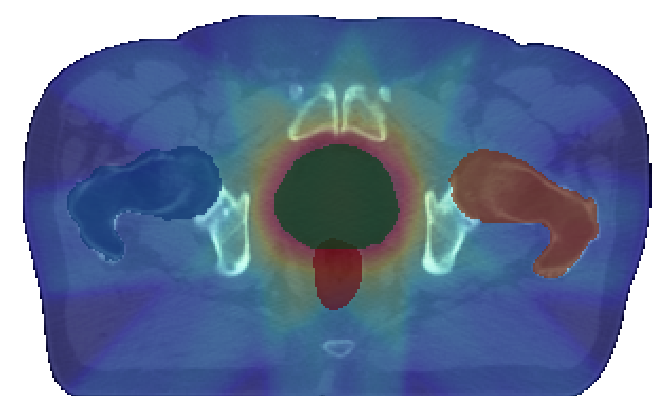
\includegraphics[width=0.5\textwidth]{example_image.pdf}
    \caption{
        CT image of a prostate cancer patient including the dose distribution of the respective treatment plan shown as iso dose lines. Areas of high dose deposition are displayed in red and orange. Contours of OAR as well as PTV are displayed in white.
        }\label{fig:prostate_oar}
\end{figure}

\subsection{MR Linear Accelerator}

In the current state of the MR-Linac employment the use of a conventional \ac{CT} as the base for treatment planning is inevitable.
On the base of this \acs{CT} target volumes and \ac{OAR} are defined by an oncologist.
In a conventional setting, this delineation and the respective treatment plan is used for all treatment fractions.
This results in uncertainties during treatment because it is assumed that the position of organs remains constant during the entire course of treatment.
Especially for moving \acs{OAR} such as bladder or sigmoid in the case of a lower abdomen cancer patient this poses a problem because it cannot be assured that they did not move during treatment or between fractions without a control \acs{CT}.
The MR-Linac offers the acquisition of an MR image before treatment.
With such position verification using an MR image the attending oncologist can decide whether previous delineations are still valid or not. If the delineations are not valid for the current fraction the MR-Linac offers a solution to adapt the treatment plan to interfraction movement of target volume or \acs{OAR}.
\acs{OAR} are registered from the CT onto the MR image and the treatment plan can be adapted to change in position or shape.
Ongoing studies investigate if this treatment modality may allow to reduce safety margins accounting for uncertainties regarding patient positioning as well as tissue movement.\\
Current research is going towards the further exploration of opportunities involving the MR-Linac.
The vision behind the MR-Linac would be to adapt the treatment plan based on real-time image acquisition during the treatment.
Critical steps to enable this proposed workflow are the optimization of all involved processes of the treatment planning pipeline to be applicable in real-time and to be based on MR images only.
An MR-only workflow is promised to ultimately result in in-time adaption to intra-fraction movements such as unwanted patient movements as well as breathing motion, potentially leading to a significant decrease in safety margins.
All necessary steps to be automated or optimized would be the delineation of tumor volumes and \acs{OAR} on MR images, treatment planning and optimization as well as pseudo-CT creation from MR images to enable \acs{DD} calculations.
Pseudo-CT creation is needed for \acs{DD} because \acs{MRI} is not a quantitative imaging modality, meaning that the pixel values of MR images are not correlated to the electron density of the tissue, which are needed for dose calculation algorithms.
Therefore a translation from qualitative MRI data to quantitative electron density information is needed to estimate deposited dose inside a given volume or patient's anatomy.\\
\acs{DD} is the part of the MR-only treatment pipeline we are focusing on in this study, trying to optimize its computational resources as well as computation time. 
As previoulsy mentioned \acs{MC} simulations are used for the simulation of particle histories to give an estimate of deposited dose inside the patient's anatomy.
These \acs{MC} simulations are used in the secondary dose calculation for treatment plan optimization as well as the dose verification.

\subsection{Physical Fundamentals}

Photons irradiated from the linear accelerator interact with the patient's tissue.
All interaction processes are of stochastic nature, meaning it can not be exactly determined when a particle will interact in which manner during its path through a dense volume.
Interaction processes of photons as well as electrons are quantitatively well described in literature, yielding probability distributions for different energies as well as tissue densities.
Main interaction processes of photons in the energy sprectrum of the MR-Linac are elastic and inelastic interactions such as rayleigh scattering, the photo effect or compton scattering, which leads to small changes in trajectory of photons inside a medium.
With increased depth inside tissue this change in trajectory leads to a widening of the initial beam.
During the latter two interaction processes photons transmit all or part of their energy onto secondary electrons.
Shorter mean free lengths and higher ionization capabilities of electrons lead to dose deposition in the nearby surrounding tissue, which is the main contribution to \acs{DD}.\\
\ac{MRI} requires a strong magnetic field. 
This magnetic field is present at all times, due to the need of superconduction. 
Trajectories of moving charged particles such as electrons are affected by the Lorentz-Force first described by \citeauthor{lorentz_versuch_1937} in \citeyear{lorentz_versuch_1937}~\cite{lorentz_versuch_1937}.
Changes in trajectory induce a shift in the \acs{DD} towards the direction of the Lorentz-Force.
Electrons have increased mean free path lengths inside low density mediums such as air compared to higher density mediums such as tissue or bones.
At the intersection of tissue to air cavities inside the patient's anatomy the Lorentz-Force influences the trajectory of electrons which causes them to return to the surface of the tissue resulting in an increase in deposited dose.
This occurence is the so called \ac{ERE}~\cite{lee_using_2017} and has significant impact on tumor sides where air cavities are present.


\subsection{Dose Deposition Calculation}

There exist multiple algorithms besides \acs{MC} for \acs{DD} that are used in reasearch and a clinical setting such as collapsed cone~\cite{ahnesjo_collapsed_1989} or pencil beam algorithms~\cite{mohan_differential_1986} which is currently used as a primary dose estimation algorithm in the institutional planning software.
In this study we focused on the \acs{MC} simulation algorithm which will build the gold standard of our dose distributions for our training data.\\
As previously mentioned, \acs{IMRT} plans are composed of individual segments for certain irradiation angles determined by the planning algorithm.
More challenging positions of target volumes and \acs{OAR} result in higher number of segments, because sparing of organs at risk becomes harder while maintaining dose coverage in the target volume, with fewer and bigger fields. 
Each segment is assigned an individual \acs{MLC} configuration, adapted to the shape of \acs{OAR} and the target volume as well as a defined number of irradiated particles.
The \acs{MLC} of a MR-Linac is composed of 80 leaf pairs of width 7.15~mm in the isocenter resulting in a maximum fieldsize of $57.2~cm \times 22~cm$.
The number of irradiated particles is measured in \ac{MU}.
100 \acs{MU} are defined as 1 Gy in depth of 10~cm inside a water phantom with a fieldsize of $10 \times 10~cm$ and a source surface distance of 100~cm.\\
To calculate the \acs{DD} for our training data, we utilized the open source software \acs{MC} solution EGSnrc~\cite{noauthor_nrc-cnrcegsnrc_2021} provided under (\citeurl{noauthor_nrc-cnrcegsnrc_2021}).
With the use of EGSnrc we were able to calculate the deposited dose for all segments indivudually. 
Previous work from our institution by \citeauthor{friedel_development_2019}~\cite{friedel_development_2019}, where the use of EGSnrc for the MR-Linac was investigated, enabled us to accurately predict the deposited dose for any beam configuration. 
The output yielded by EGSnrc is normalized to 100~\acs{MU} for the given input parameters such as irradiation volume and accelerator settings.\\

\acs{MC} simulations such as EGSnrc are used for dose calculation in both clinical and research applications.
Photons transfer their energy in the irradiated volume to electrons or positrons in the energy spectrum of interest for external beam radiotherapy. 
In the absence of an analytical solution, without significant simplifications and assumptions for the conditions, the \acs{MC} algorithm is used to simulate a variety of particle trajectories in the desired target volume.
Particle trajectories describe the precise path of a photon from the source to the point in the volume where it has lost all of its energy, including energy tranfer to secondary electrons in the course of collisions.
The stochastic nature of the interaction processes of photons and electrons requires a large number of simulated particles to obtain an accurate result. 
Long simulation times are the consequence with a number of histories on the order of 10\textsuperscript{7} to 10\textsuperscript{11}.